\documentclass{beamer}

\usepackage{lmodern}
\usepackage[utf8]{inputenc}

\usetheme{Berlin}
\usecolortheme{seagull}

\title{Fitting Two Point Clouds From 3D Scans}
\author{Rodrigo Caye Daudt,\\ Mr. Kaisar,\\ Mr. Sepehr}
\institute{Université de Bourgogne}
\date{January 2016}


\begin{document}


\frame{\titlepage}

\begin{frame}
\frametitle{ICP}

\begin{figure}[H]
\centering
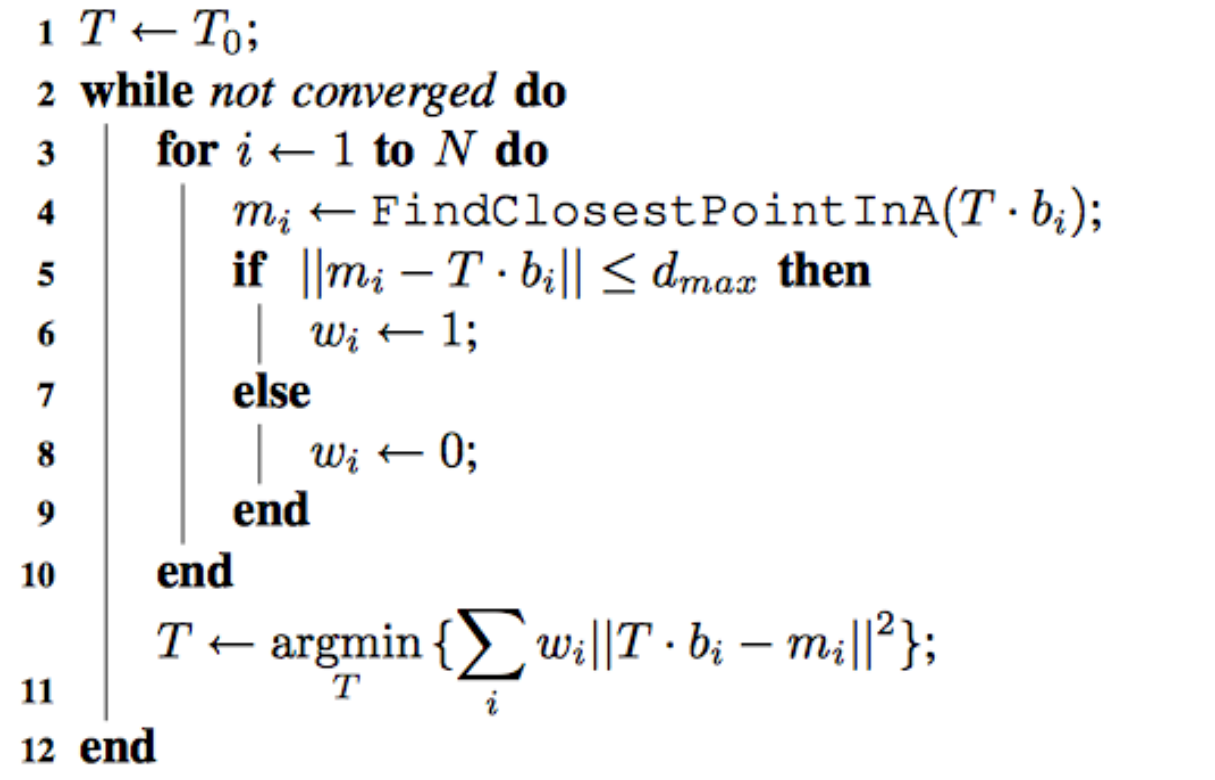
\includegraphics[width=4in]{figures/04-ICP.png}
\end{figure}

\end{frame}


\begin{frame}
\frametitle{Point clouds}

\begin{figure}[H]
\centering
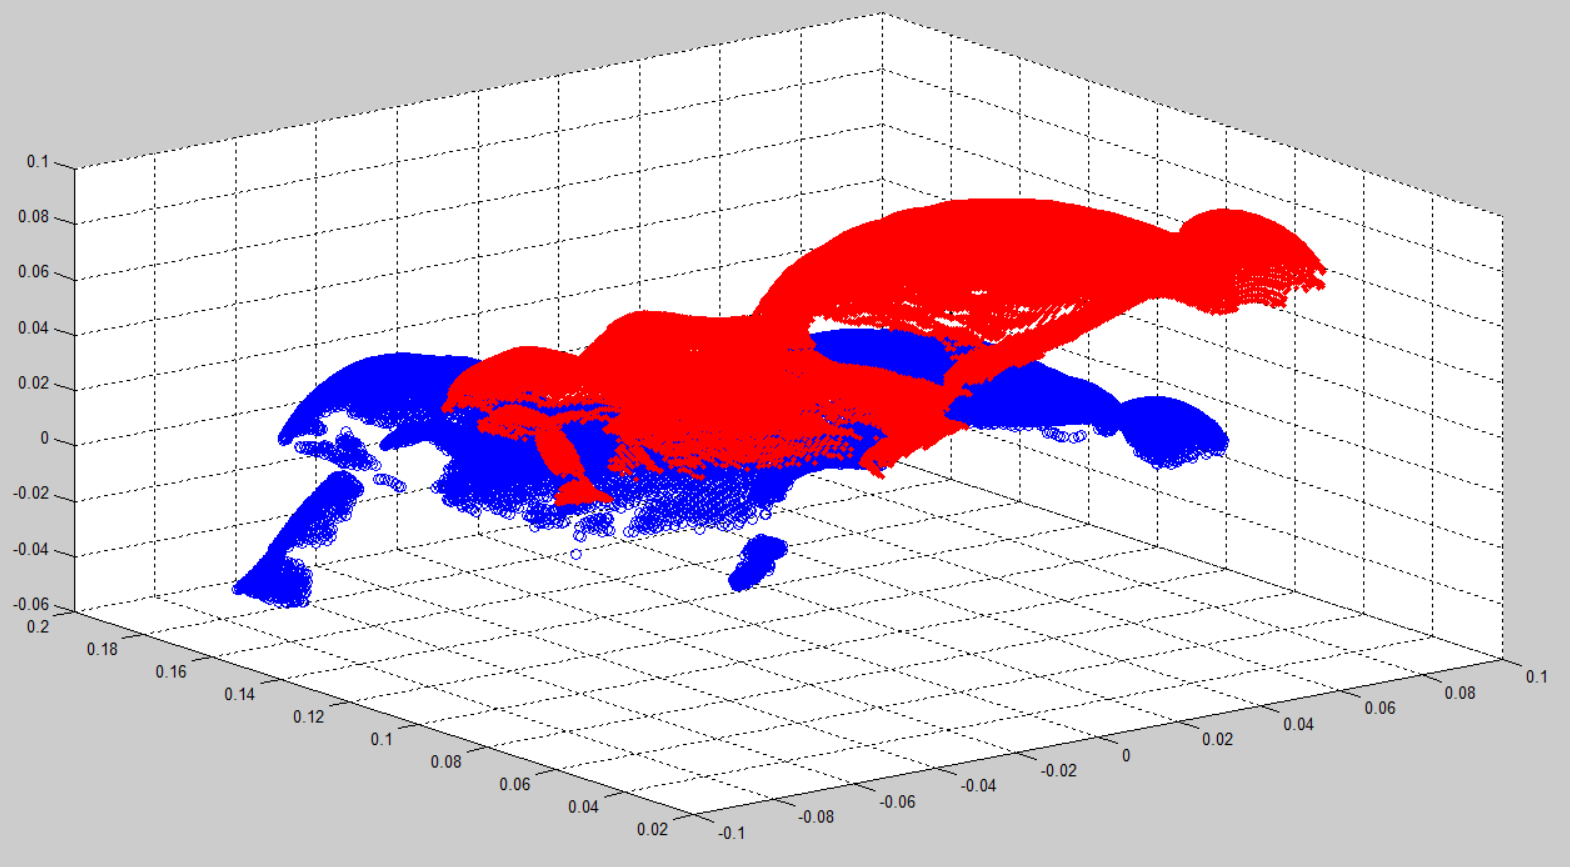
\includegraphics[width=4in]{figures/01-bunnies.png}
\end{figure}

\end{frame}


\begin{frame}
\frametitle{Point clouds after fitting}

\begin{figure}[H]
\centering
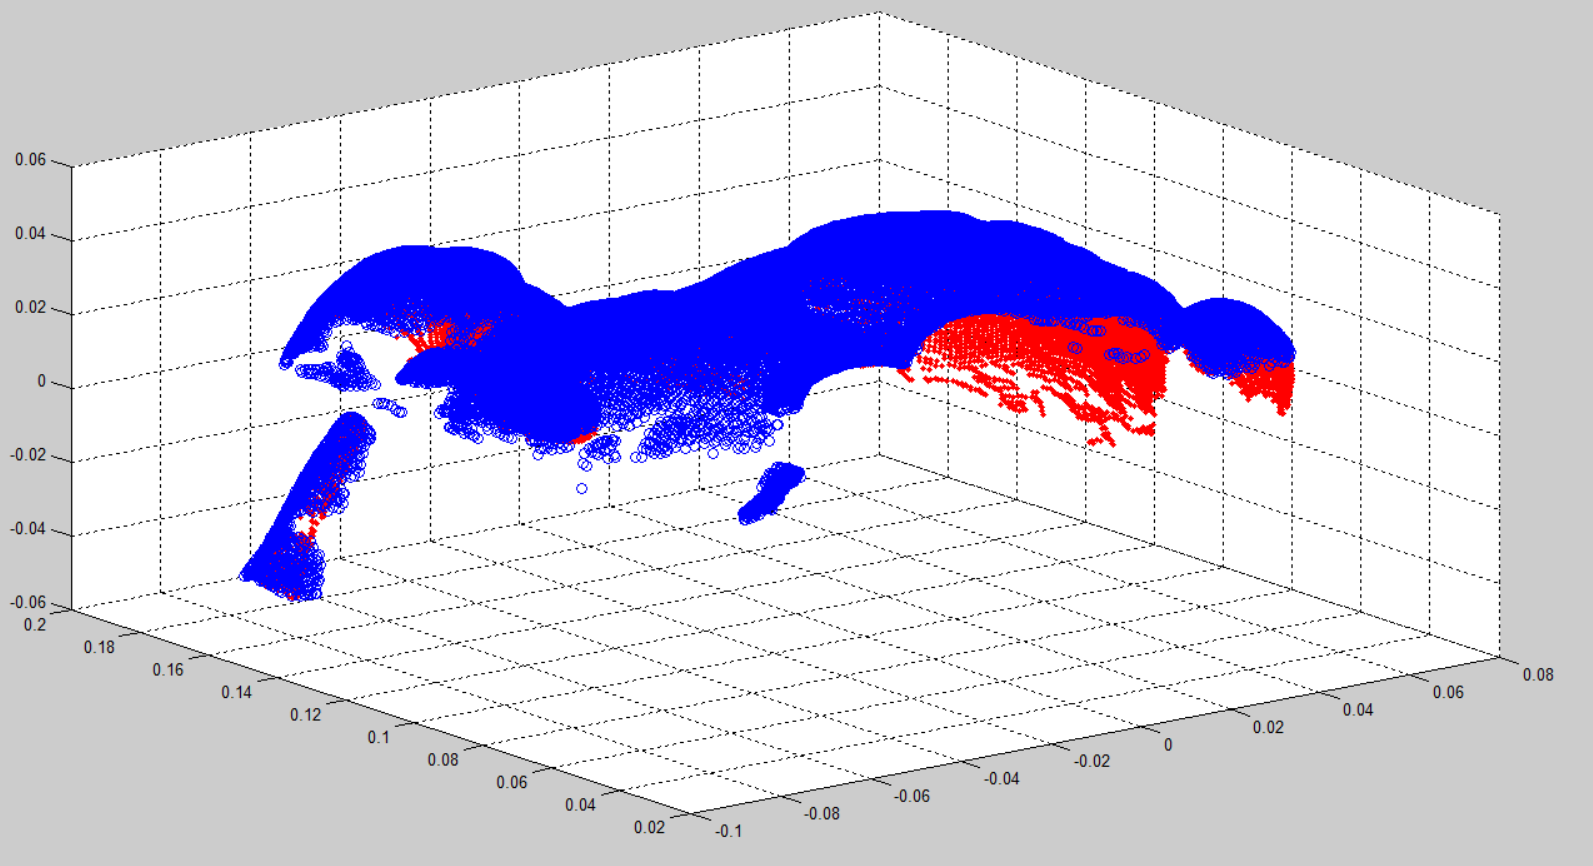
\includegraphics[width=4in]{figures/02-fittedBunnies.png}
\end{figure}

\end{frame}


\begin{frame}
\frametitle{Plot of error over iterations}

\begin{figure}[H]
\centering
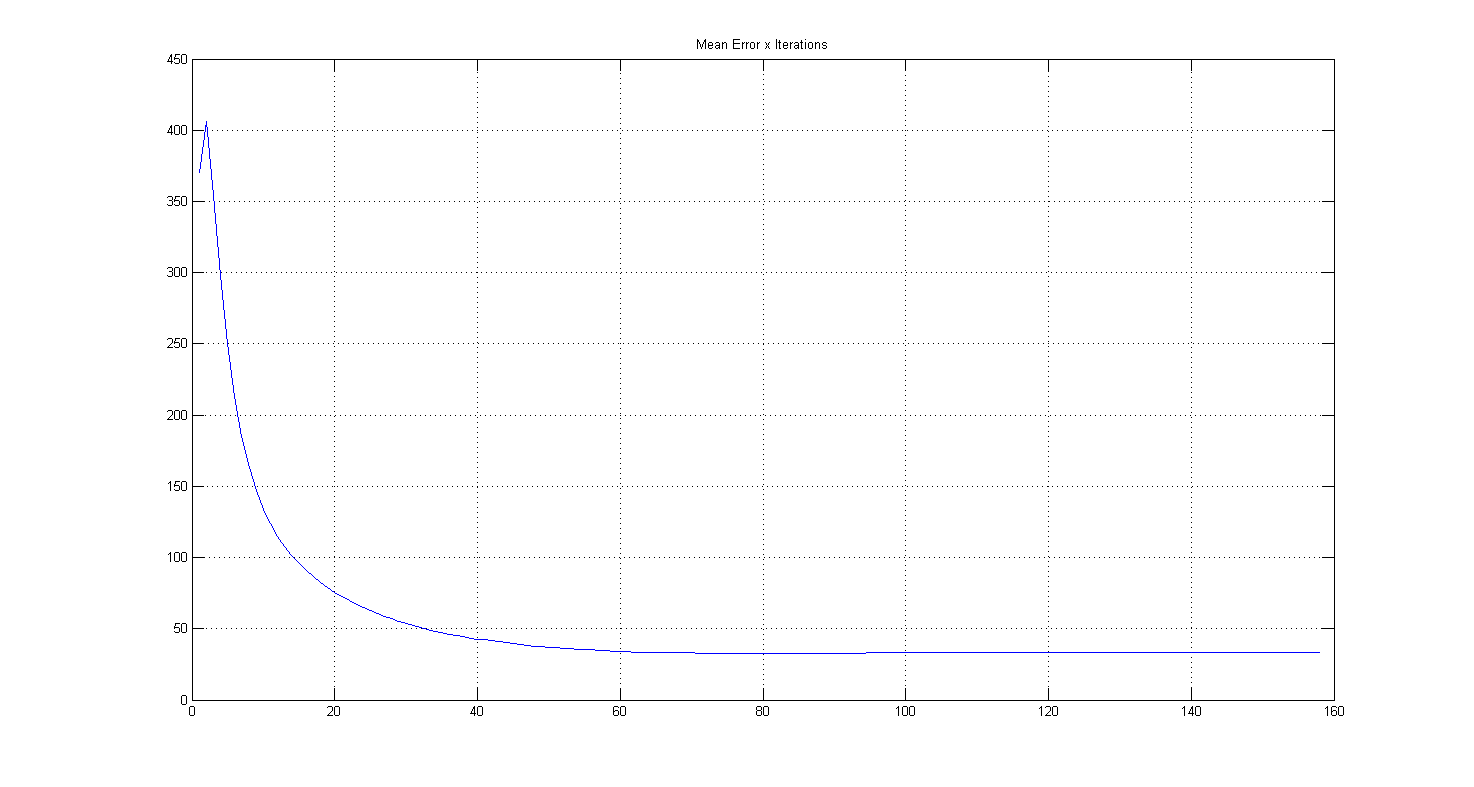
\includegraphics[width=4in]{figures/03-MeanErrorPlot.png}
\end{figure}

\end{frame}




\end{document}
